%%%%%%%%%%%%%%%%%%%%%%%%%%%%%%%%%%%%%%%%%
% Short Sectioned Assignment
% LaTeX Template
% Version 1.0 (5/5/12)
%
% This template has been downloaded from:
% http://www.LaTeXTemplates.com
%
% Original author:
% Frits Wenneker (http://www.howtotex.com)
%
% License:
% CC BY-NC-SA 3.0 (http://creativecommons.org/licenses/by-nc-sa/3.0/)
%
%%%%%%%%%%%%%%%%%%%%%%%%%%%%%%%%%%%%%%%%%

%----------------------------------------------------------------------------------------
%	PACKAGES AND OTHER DOCUMENT CONFIGURATIONS
%----------------------------------------------------------------------------------------

\documentclass[paper=a4, fontsize=11pt]{scrartcl} % A4 paper and 11pt font size

\usepackage[T1]{fontenc} % Use 8-bit encoding that has 256 glyphs
\usepackage{fourier} % Use the Adobe Utopia font for the document - comment this line to return to the LaTeX default
\usepackage[english]{babel} % English language/hyphenation
\usepackage{amsmath,amsfonts,amsthm,amssymb,mathtools} % Math packages
\usepackage{atbegshi,picture} %atBeginShipout for boxed name at top
%\AtBeginShipoutNext{\AtBeginShipoutUpperLeft{%next makes just first page
%  \put(\dimexpr\paperwidth-1cm\relax,-1.9cm){\makebox[0pt][r]{\framebox{Keegan J Kell --- $keeganjk$}}}%
%}}

%\DeclarePairedDelimiter{\ceil}{\lceil}{\rceil}
%\DeclarePairedDelimiter{\flrr}{\lceil}{\rceil}

\usepackage{lipsum} % Used for inserting dummy 'Lorem ipsum' text into the template

\usepackage{sectsty} % Allows customizing section commands
\allsectionsfont{\centering \normalfont\scshape} % Make all sections centered, the default font and small caps

\usepackage{fancyhdr} % Custom headers and footers
\pagestyle{fancyplain} % Makes all pages in the document conform to the custom headers and footers
\fancyhead{} % No page header - if you want one, create it in the same way as the footers below
\fancyfoot[L]{} % Empty left footer
\fancyfoot[C]{} % Empty center footer
\fancyfoot[R]{\thepage} % Page numbering for right footer
\renewcommand{\headrulewidth}{0pt} % Remove header underlines
\renewcommand{\footrulewidth}{0pt} % Remove footer underlines
\setlength{\headheight}{13.6pt} % Customize the height of the header

\numberwithin{equation}{section} % Number equations within sections (i.e. 1.1, 1.2, 2.1, 2.2 instead of 1, 2, 3, 4)
\numberwithin{figure}{section} % Number figures within sections (i.e. 1.1, 1.2, 2.1, 2.2 instead of 1, 2, 3, 4)
\numberwithin{table}{section} % Number tables within sections (i.e. 1.1, 1.2, 2.1, 2.2 instead of 1, 2, 3, 4)

\setlength\parindent{0pt} % Removes all indentation from paragraphs - comment this line for an assignment with lots of text



%----------------------------------------------------------------------------------------
%	TITLE SECTION
%----------------------------------------------------------------------------------------

\newcommand{\horrule}[1]{\rule{\linewidth}{#1}} % Create horizontal rule command with 1 argument of height

\title{	
\normalfont \normalsize 
\textsc{Institute of Technology} \\ [25pt] % Your university, school and/or department name(s)
\horrule{0.5pt} \\[0.4cm] % Thin top horizontal rule
\huge TCSS 360 - Iteration 1 \\ % The assignment title
\horrule{2pt} \\[0.5cm] % Thick bottom horizontal rule
}

\usepackage{fancyhdr}
\pagestyle{fancy}
%\addtolength{\headwidth}{\marginparsep} %these change header-rule width
%\addtolength{\headwidth}{\marginparwidth}
\lhead{}
\chead{} 
\rhead{}
\lfoot{Energy Saver --- TCSS 360B Spring 2017}
\cfoot{} 
\rfoot{\thepage} 
\setlength{\headheight}{15pt}
\renewcommand{\headrulewidth}{.3pt} 
\renewcommand{\footrulewidth}{.3pt}
\setlength\voffset{-0.25in}
\setlength\textheight{648pt}
\setlength{\parindent}{0pt}
\setlength{\parskip}{1ex plus 0.5ex minus 0.2ex}

%%\author{\normalsize \textit keeganjk \\ Keegan Kell} % Your name
\date{April 16, 2017} % Today's date or a custom date

\begin{document}

\maketitle % Print the title

%----------------------------------------------------------------------------------------
%	PROBLEM 1
%----------------------------------------------------------------------------------------
\thispagestyle{empty}
\section{Team Energy Saver}
\begin{center}
Alex Smith --- $asmith58$\\
Darren Carpenter --- $carpedar$\\
Nikolai Carlson --- $nmc37$\\
Keegan Kell --- $keeganjk$\\
Lola Howell --- $lola2010$\\
\end{center}

$$https://energysaverweb.wordpress.com$$
$$diyenergysaver@gmail.com$$

\clearpage
\section{Running Application}
\begin{center}
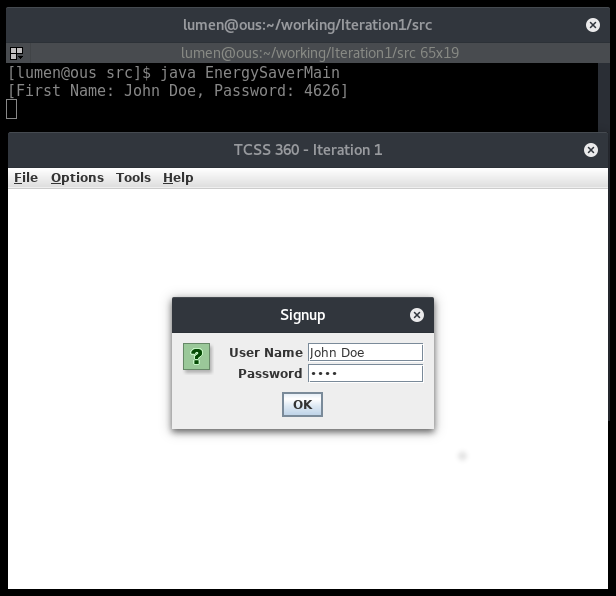
\includegraphics[scale=0.45]{signup.png}\\
$Signup$ is accessible via the $File$ menu.
\end{center}
Basic functionality is implemented for users, but some things need planned out for later:
\begin{enumerate}
\item invalid or identical name/email
\item canceling the signup procedure
\item forcing legal input on both fields upon pressing OK
\item location/type of underlying multi-user data structure
\end{enumerate}
\begin{center}
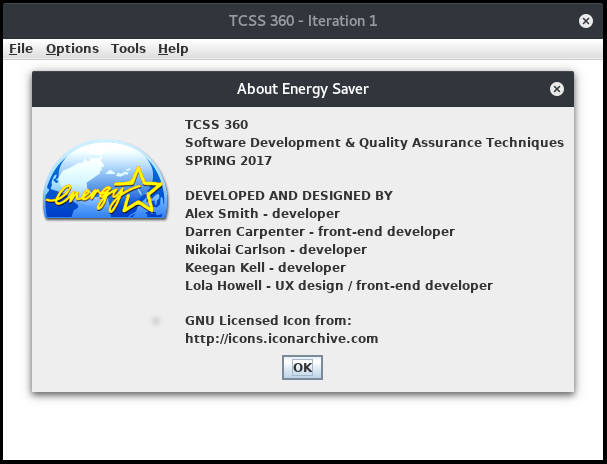
\includegraphics[scale=0.45]{about.png}\\
$About$ is accessible via the $Help$ menu.
\end{center}

\clearpage

Every group member has the basic eclipse/github setup or equivalent.  We hope to have 
everyone demonstrate code retrieval and editing by Saturday, though issues may postpone 
this until our next meeting on Tuesday.

\section{JUnit Coverage}

Current trivial tests:

\begin{enumerate}
\item tests default constructor for first name
\item tests default constructor for email
\item tests toString() of User.class
\end{enumerate}

\begin{center}
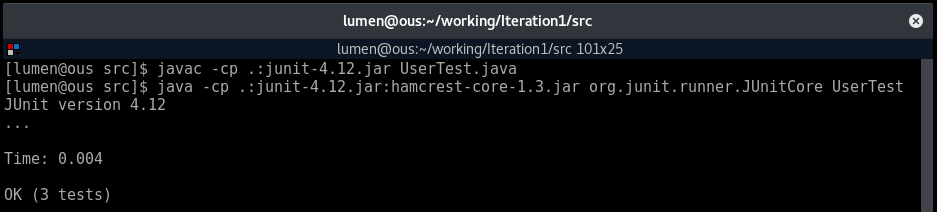
\includegraphics[scale=0.45]{junit.png}
\end{center}


\end{document}